%
% Template Laporan Skripsi/Thesis
%
% @author  Andreas Febrian, Lia Sadita
% @version 1.03
%
% Dokumen ini dibuat berdasarkan standar IEEE dalam membuat class untuk
% LaTeX dan konfigurasi LaTeX yang digunakan Fahrurrozi Rahman ketika
% membuat laporan skripsi. Konfigurasi yang lama telah disesuaikan dengan
% aturan penulisan thesis yang dikeluarkan UI pada tahun 2008.
%

%
% Disesuaikan untuk template skripsi/tesis UIN K.H. Abdurrahman Wahid
% Pekalongan
% @author Slamet B. Aryo
%

%
% Tipe dokumen adalah report dengan satu kolom.
%
\documentclass[12pt, a4paper, onecolumn, oneside, final]{report}
%\raggedbottom

% Load konfigurasi khusus untuk laporan yang sedang dibuat
%-----------------------------------------------------------------------------%
% Informasi Mengenai Dokumen
%-----------------------------------------------------------------------------%
%
% Perintah untuk membuat perintah/variabel baru.
\newcommand{\var}[2]{\newcommand{#1}{#2}}
%
% Perintah untuk membuat perintah/variabel baru. Teks yang ditulis dalam
% perintah ini akan diformat ulang menggunakan huruf kapital.
\newcommand{\Var}[2]{\newcommand{#1}{\uppercase{#2}}}
%
% Judul laporan.
\var{\judul}{Judul Karya Ilmiah Anda}
%
% Tulis kembali judul laporan, kali ini akan diubah menjadi huruf kapital
\Var{\Judul}{Judul Karya Ilmiah Anda}
%
% Tulis kembali judul laporan namun dengan bahasa Ingris
\var{\judulInggris}{Your Scientific Publication Title}
%
% Nama tempat penelitian
\var{\lokus}{Sebuah Tempat yang Diteliti}
\var{\Lokus}{SEBUAH TEMPAT YANG DITELITI}

%
% Tipe laporan, dapat berisi Skripsi, Tugas Akhir, Thesis, atau Disertasi
\var{\type}{skripsi}
%
% Tulis kembali tipe laporan, kali ini akan diubah menjadi huruf kapital
\var{\Type}{Skripsi}
%
% Tulis nama penulis
\var{\penulis}{Nama Lengkap Anda}
%
% Tulis kembali nama penulis, kali ini akan diubah menjadi huruf kapital
\Var{\Penulis}{Nama Lengkap Anda}
%
% Tulis NPM / NIM penulis
\var{\npm}{Nomor Anda}
\var{\nim}{Nomor Anda}
%
% Tuliskan Fakultas dimana penulis berada
\Var{\Fakultas}{Fakultas Anda}
\var{\fakultas}{Fakultas Anda}
\var{\websiteFakultas}{www.febi.uingusdur.ac.id}
\var{\emailFakultas}{febi@uingusdur.ac.id}
%
% Tuliskan Program Studi yang diambil penulis
\Var{\Program}{Jurusan Anda}
\var{\program}{Jurusan Anda}
%
% Tuliskan tahun publikasi laporan
\Var{\bulanTahun}{Bulan Tahun}
\Var{\tahun}{2022}
%
% Tuliskan gelar yang akan diperoleh dengan menyerahkan laporan ini
\var{\gelar}{Gelar Jurusan Anda}
%
\var{\tanggalSeminarProp}{Tanggal Bulan Tahun}
% Tuliskan tanggal pengesahan laporan, waktu dimana laporan diserahkan ke
% penguji/sekretariat
\var{\tanggalPengesahanProposal}{Tanggal Bulan Tahun}
\var{\tanggalSiapSidang}{Tanggal Bulan Tahun}
%
% Tuliskan tanggal keputusan sidang dikeluarkan dan penulis dinyatakan
% lulus/tidak lulus
\var{\tanggalLulus}{Tanggal Bulan Tahun}
\var{\hariLulus}{Hari}
% Tuliskan tanggal pengesahan laporan final, waktu dimana laporan
% diserahkan ke perpustakaan
\var{\tanggalFinal}{Tanggal Bulan Tahun}
% sama dengan tanggal final
\var{\tanggalPengesahan}{Tanggal Bulan Tahun}
%
% Tuliskan pembimbing
\var{\pembimbingSatu}{Pembimbing Pertama Anda}
\var{\nipPembimbingSatu}{1234567890}
\var{\pembimbingDua}{Pembimbing Kedua Anda}
\var{\nipPembimbingDua}{1234567890}
%
% Tuliskan penguji
\var{\pengujiSatu}{Penguji Pertama Anda}
\var{\nipPengujiSatu}{1234567890}
\var{\pengujiDua}{Penguji Kedua Anda}
\var{\nipPengujiDua}{1234567890}

%-----------------------------------------------------------------------------%
% Judul Setiap Bab
%-----------------------------------------------------------------------------%
%
% Berikut ada judul-judul setiap bab.
% Silahkan diubah sesuai dengan kebutuhan.
%
\var{\kataPengantar}{Kata Pengantar}
\var{\babSatu}{PENDAHULUAN}
\var{\babDua}{LANDASAN TEORI}
\var{\babTiga}{METODE PENELITIAN}
\var{\babEmpat}{ANALISIS DATA DAN PEMBAHASAN}
\var{\babLima}{Pendalaman}
\var{\kesimpulan}{PENUTUP}
%
% Untuk abstrak
\var{\subjekpen}{Wakaf Uang, Pengelolaan Dana, dan Efektivitas Distribusi Dananya}
\var{\abstrak}{Wakaf uang adalah dana yang ditahan untuk dimanfaatkan secara berkesinambungan}
%
% Nama-nama narasumber dalam wawancara
\var{\narsumSatu}{Bapak Narasumber Pratama}
\var{\narsumDua}{Ibu Narasumber Zwei}
\var{\narsumTiga}{Bapak Narasumber Tri}


% pdfa xmp
\begin{filecontents*}[overwrite]{\jobname.xmpdata}
  \Title{\judul}
  \Author{\penulis}
  \Language{id-ID}
  \Subject{\subjekpen}
  \Keywords{kata satu\sep kunci dua\sep kata kunci tiga}
\end{filecontents*}

% Load konfigurasi LaTeX untuk tipe laporan thesis
\usepackage{etc/uithesis}

% Daftar pemenggalan suku kata dan istilah dalam LaTeX
%
% Hyphenation untuk Indonesia 
%
% @author  Andreas Febrian
% @version 1.00
% 
% Tambahkan cara pemenggalan kata-kata yang salah dipenggal secara otomatis 
% oleh LaTeX. Jika kata tersebut dapat dipenggal dengan benar, maka tidak 
% perlu ditambahkan dalam berkas ini. Tanda pemenggalan kata menggunakan 
% tanda '-'; contoh:
% menarik
%   --> pemenggalan: me-na-rik
%

\hyphenation{
    % alphabhet A
    a-na-li-sa a-tur 
    a-pli-ka-si 
    % alphabhet B
    ba-ngun-an 
    be-be-ra-pa 
    ber-ge-rak
    ber-ke-lan-jut-an 
    ber-pe-nga-ruh 
    % alphabhet C
    ca-ri
    % alphabhet D
    di-da-pat-kan di-sim-pan di-pim-pin de-ngan da-e-rah di-ba-ngun da-pat di-nya-ta-kan 
    di-sim-bol-kan di-pi-lih di-li-hat de-fi-ni-si di-de-fi-ni-si-kan di-mi-li-ki
    % alphabhet E
    e-ner-gi eks-klu-sif
    % alphabhet F
    fa-si-li-tas
    % alphabhet G
    ga-bung-an ge-rak
    % alphabhet H
    ha-lang-an
    % alphabhet I
    % alphabhet J
    % alphabhet K
    ke-hi-lang-an
    ku-ning 
    kua-li-tas ka-me-ra ke-mung-kin-an ke-se-pa-ham-an
    % alphabhet L
    ling-kung-an
    % alphabhet M
    me-neng-ah
    meng-a-tas-i me-mung-kin-kan me-nge-na-i me-ngi-rim-kan 
    meng-u-bah meng-a-dap-ta-si me-nya-ta-kan mo-di-fi-ka-si
    meng-a-tur meng-a-rah-kan mi-lik
    % alphabhet N
    nya-ta non-eks-klu-sif
    % alphabhet O
    % alphabhet P
	pe-nye-rap-an 
	pe-ngon-trol
    pe-mo-del-an
    pe-ran  pe-ran-an-nya
    pem-ba-ngun-an pre-si-den pe-me-rin-tah prio-ri-tas peng-am-bil-an 
    peng-ga-bung-an pe-nga-was-an pe-ngem-bang-an 
    pe-nga-ruh pa-ra-lel-is-me per-hi-tung-an per-ma-sa-lah-an 
    pen-ca-ri-an peng-struk-tur-an pen-ting pen-ting-nya
    % alphabhet Q
    % alphabhet R
    ran-cang-an
    % alphabhet S
    si-mu-la-si sa-ngat
    % alphabhet T
    te-ngah
    ter-da-pat
    % alphabhet U
    % alphabhet V
    va-ri-an va-ri-a-si
    % alphabhet W
    % alphabhet X
    % alphabhet Y
    % alphabhet Z
    % special
}


% Daftar istilah yang mungkin perlu ditandai
%
% @author  Andreas Febrian
% @version 1.00
%
% Mendaftar seluruh istilah yang mungkin akan perlu dijadikan
% italic atau bold pada setiap kemunculannya dalam dokumen.
%

\var{\license}{\f{Creative Common License 1.0 Generic}}
\var{\bslash}{$\setminus$}


% Awal bagian penulisan laporan
\begin{document}

\pagestyle{standard}

%
% Sampul Laporan
%
% Sampul Laporan

%
% @author  unknown
% @version 1.10
% @edit by Andreas Febrian
% @modified by Slamet B. Aryo
%

\begin{titlepage}
    \begin{center}

        \vspace*{.5cm}
        % judul thesis harus dalam 14pt Times New Roman
        {\large \bo{\Judul \\}} %\\[1.0cm]

        \vspace*{1cm}
        % harus dalam 14pt Times New Roman
        \bo{\MakeUppercase{\Type}} \\

        \vspace*{1cm}
        % keterangan prasyarat
        Diajukan untuk memenuhi sebagian syarat memperoleh gelar \\
        \gelar\\

        \vspace*{1cm}
        \begin{figure}
            \begin{center}
                
\includegraphics[width=5.22cm]{assets/pics/logo-color.ps}
            \end{center}
        \end{figure}

        \vspace*{1cm}
        % penulis dan nim
        Oleh:\\
        \underline{\bo{\Penulis}} \\
        \bo{NIM: \nim} \\

        %\vspace*{1.5cm}
        \vfill

        % informasi mengenai fakultas dan program studi
        {\large \bo{
            PROGRAM STUDI \Program \\
            FAKULTAS \Fakultas\\
            UNIVERSITAS ISLAM NEGERI\\
            K.H. ABDURRAHMAN WAHID PEKALONGAN\\
            \tahun\\
        }}
    \end{center}
\end{titlepage}

%\forceclearchapter

%
% Gunakan penomeran romawi
\pagenumbering{roman}
\pagestyle{first-pages}

%
% load halaman judul dalam
\addChapter{HALAMAN JUDUL}
%
% Halaman Judul Laporan
%
% @author  unknown
% @version 1.01
% @edit by Andreas Febrian
%

\begin{titlepage}
    \begin{center}\begin{figure}
            \begin{center}
                
\includegraphics[width=2.5cm]{assets/pics/makara.png}
            \end{center}
        \end{figure}
        \vspace*{0cm}
        \bo{
        	UNIVERSITAS INDONESIA\\
        }

        \vspace*{1.0cm}
        % judul thesis harus dalam 14pt Times New Roman
        \bo{\Judul} \\[1.0cm]

        \vspace*{2.5 cm}
        % harus dalam 14pt Times New Roman
        \bo{\Type} \\
        % keterangan prasyarat
        \bo{Diajukan sebagai salah satu syarat untuk memperoleh gelar \\
        \gelar}\\

        \vspace*{3 cm}
        % penulis dan npm
        \bo{\Penulis} \\
        \bo{\npm} \\

        \vspace*{5.0cm}

        % informasi mengenai fakultas dan program studi
        \bo{
        	FAKULTAS \Fakultas\\
        	PROGRAM STUDI \Program \\
        	DEPOK \\
        	\bulanTahun
        }
    \end{center}
\end{titlepage}

%\forceclearchapter

%
% setelah bagian ini, halaman dihitung sebagai halaman ke 2
%\setcounter{page}{2}
\doublespacing

%
% load halaman orisinalitas
\addChapter{LEMBAR PERNYATAAN KEASLIAN}
%
% Halaman Orisinalitas
%
% @author  Andreas Febrian
% @version 1.01
%

\chapter*{\uppercase{halaman pernyataan orisinalitas}}
\vspace*{2cm}

\begin{center}
	\bo{\type~ini adalah hasil karya saya sendiri, \\
	dan semua sumber baik yang dikutip maupun dirujuk \\
	telah saya nyatakan dengan benar.} \\
	\vspace*{2.6cm}

	\begin{tabular}{l c l}
	\bo{Nama} & : & \bo{\penulis} \\
	\bo{NPM} & : & \bo{\npm} \\
	\bo{Tanda Tangan} & : & \\
	& & \\
	& & \\
	\bo{Tanggal} & : & \bo{\tanggalSiapSidang} \\
	\end{tabular}
\end{center}

\newpage

%% file keaslian pdf hasil scan yang memuat tanda tangan
% \putpdf{submission/pernyataan-keaslian}
%\forceclearchapter
%
% load halaman nota pembimbing
\addChapter{LEMBAR NOTA PEMBIMBING}
%
% Halaman Pengesahan
%
% @author  Andreas Febrian
% @version 1.01
%

\chapter*{HALAMAN PERSETUJUAN}

\vspace*{0.2cm}
\noindent

\noindent
\begin{tabular}{l l p{11cm}}
	\bo{Judul}&: & \judul \\
	\bo{Nama}&: & \penulis \\
	\bo{NPM}&: & \npm \\
\end{tabular} \\

\vspace*{1.2cm}

\noindent Laporan \type~ini telah diperiksa dan disetujui.\\[0.3cm]
\begin{center}
\tanggalFinal \\[2cm]
\end{center}

\begin{center}
\begin{multicols}{2}
\underline{\pembimbingSatu}\\[0.1cm]
Pembimbing \type

\underline{\pembimbingDua}\\[0.1cm]
Pembimbing \type
\end{multicols}
\end{center}

\newpage

% file discan
% \putpdf{submission/nota-bimbing-skrip}
%\forceclearchapter
%\clearpage
%
% \enlargethispage{-7\baselineskip}
\addChapter{LEMBAR PENGESAHAN}
%
% Halaman Pengesahan Sidang
%
% @author  Andreas Febrian, Andre Tampubolon
% @author  Slamet B. Aryo
% @version 1.10
%
\BgThispage
% \thispagestyle{kopkampus}
% \enlargethispage{3\baselineskip}
% \vspace*{-10\baselineskip}
\vspace*{-2\baselineskip}

% kop terinspirasi dari
% https://www.overleaf.com/latex/templates/letterhead/zkvhmkzskgdm

\begin{figure}[!ht]
%\begin{minipage}{\textwidth}
\begin{center}
\begin{spacing}{.85}
\begin{tabular}[t]{l c}
\multirow{5}{*}{
\includegraphics[width=0.15\linewidth]{assets/pics/logo-color.ps}} &
\bo{KEMENTERIAN AGAMA REPUBLIK INDONESIA}  \\
& \small{\bo{UNIVERSITAS ISLAM NEGERI}} \\
& \small{\bo{K.H. ABDURRAHMAN WAHID PEKALONGAN}} \\
& \small{\bo{FAKULTAS \Fakultas}} \\
& \scriptsize{Jalan Pahlawan No. 52 Rowolaku Kajen, Pekalongan Tlp. (0285) 412575, Fax. (0285) 423418} \\
& \scriptsize{Website: \websiteFakultas\ Email: \emailFakultas} \\
\end{tabular}

% gambar garis kop
\hrule width \hsize \kern 0.5mm \hrule width \hsize height 2pt
\end{spacing}
\end{center}
%\end{minipage}
\end{figure}

\vspace*{-1cm}

% \chapter*{P E N G E S A H A N}
\begin{center}
{\textbf{P E N G E S A H A N}}
\end{center}

\vspace*{0.4cm}

Dekan Fakultas \fakultas\ Universitas Islam Negeri (UIN) K.H. Abdurrahman Wahid Pekalongan mengesahkan \type\ Saudara/i:\\

\noindent
\begin{tabularx}{\linewidth}{@{}l l @{\hspace{.5em}}X@{}}
	%\type~ini diajukan oleh&: & \\
	Nama&: & \bo{\penulis} \\
	NIM&: & \bo{\nim} \\
	%Jurusan&: & \program \\
	Judul \Type&: & \bo{\judul} \\
        Dosen Pembimbing&: & \bo{\pembimbingSatu} \\
\end{tabularx} \\

\vspace*{0.5em}

%Telah diujikan pada hari ............. tanggal .......................... dan dinyatakan
Telah diujikan pada hari \hariLulus~tanggal \tanggalLulus~dan dinyatakan
\bo{\underline{LULUS}} serta diterima sebagai salah satu syarat guna
memperoleh gelar \gelar.%\\[0.2cm]

\begin{center}
	Dewan Penguji,
\end{center}

\vspace*{-1cm}


\begin{center}

\columnratio{0.4} %rasio kolom kiri dan kanan, untuk menyesuaikan jika nama dosen terlalu panjang
\begin{paracol}{2}
Penguji I\\[3em]
\underline{\bo{\pengujiSatu}}\\[-0.6em]
NIP. \nipPengujiSatu

\switchcolumn

Penguji II\\[3em]
\underline{\bo{\pengujiDua}}\\[-0.6em]
NIP. \nipPengujiDua
\end{paracol}

%Pekalongan, ........................\\[-0.6em]
Pekalongan, \tanggalLulus\\[-0.6em]
Dekan Fakultas \fakultas\\[3em]

\underline{\bo{Prof. Dr. Nama Dekan}}\\[-0.6em]
NIP. 1234567890
\end{center}


\newpage

%\forceclearchapter
%\clearpage
%
%
%\pagestyle{standard}
\setcounter{page}{5}
\addChapter{LEMBAR MOTTO}
%
% Halaman Lembar Motto
%
% @author  Slamet B. Aryo
% @version 1.01
%
\chapter*{MOTTO}

\vspace{2cm}
\begin{center}
\textit{
``Happiness comes from solving problems.''\\
(Mark Manson)
}

\vspace{2cm}
\textit{
``Becik ketitik ala ketara.''\\
(Adagium Jawa)
}
\end{center}

\newpage


%\forceclearchapter
%
%
\addChapter{LEMBAR PERSEMBAHAN}

\chapter*{PERSEMBAHAN}

Puji syukur kehadirat Allah SWT yang telah memberikan limpahan nikmat dan karunia-Nya
sehingga penulis dapat menyelesaikan \type~ini. \Type~ini disusun untuk memenuhi persyaratan
dalam memperoleh gelar \gelar~ di Universitas Islam Negeri K.H. Wahid Hasyim.
Penulis menyadari sepenuhnya atas segala keterbatasan dan banyaknya kekurangan-kekurangan
yang harus diperbaiki dalam penulisan \type~ini.
Semoga hasil penelitian ini dapat memberikan informasi dan manfaat bagi setiap orang
yang membacanya, khususnya bagi dunia pendidikan.
Dalam pembuatan \type~ini penulis banyak mendapatkan berbagai dukungan serta bantuan materiil
maupun non materiil dari berbagai pihak.
Berikut ini pihak-pihak yang telah berperan dalam membantu terlaksananya penulisan \type~ini:

\begin{enumerate}
 \item{Kedua orang tua tercinta\ldots}
 \item{Keluarga\ldots}
 \item{Almamater saya jurusan \program, Fakultas \fakultas~UIN Gusdur\ldots}
 \item{Dosen pembimbing\ldots}
 \item{Dosen Wali\ldots}
 \item{Sahabat\ldots}
 \item{Teman-teman\ldots}
 \item{Dll.}
\end{enumerate}


\newpage


%
%
\addChapter{ABSTRAK}
%
% Halaman Abstract
%
% @author  Andreas Febrian
% @version 1.00
%

\chapter*{ABSTRACT}
%\singlespacing

\vspace*{0.2cm}

\noindent \begin{tabular}{l l p{11.0cm}}
	Name&: & \penulis \\
	Program&: & \program \\
	Title&: & \judulInggris \\
\end{tabular} \\

\vspace*{0.5cm}

\noindent Abstract content. \\

\vspace*{0.2cm}

\noindent \bo{Key words:} \\ Keyword one, keyword two \\

%\onehalfspacing
\newpage

%
\addChapter{\MakeUppercase{\kataPengantar}}
%
% Halaman Pengantar
%
% @author  Andreas Febrian
% @author  Slamet B. Aryo
% @version 1.01
%
%-----------------------------------------------------------------------------%
\chapter*{\kataPengantar}
%-----------------------------------------------------------------------------%

Puji syukur penulis ucapkan kepada Tuhan Yang Maha Esa, karena atas berkat
dan rahmat-Nya dapat menyelesaikan \type~ini.
Penulisan \type~ini dilakukan dalam rangka memenuhi salah satu syarat untuk
mencapai gelar \gelar~Jurusan \program~pada Fakultas \fakultas~UIN Gusdur.
Penulis menyadari bahwa tanpa bantuan dan bimbingan dari berbagai pihak,
dari masa perkuliahan sampai pada penyusunan \type~ini, sangatlah sulit bagi
penulis untuk menyelesaikan \type~ini.
Oleh karena itu, penulis mengucapkan terima kasih kepada:
\begin{enumerate}[topsep=0pt,itemsep=-1ex,partopsep=1ex,parsep=1ex]
	\item Dr.\ldots selaku Rektor UIN Gusdur.
	\item Dr.\ldots selaku Dekan \fakultas.
	\item Dr.\ldots selaku Wakil Dekan bidan Akademik dan Kelembagaan \fakultas.
	\item Dr.\ldots selaku Ketua Jurusan \program.
	\item Dr.\ldots selaku Sekretaris Jurusan \program.
	\item Dr.\ldots selaku dosen pembimbing yang telah menyediakan waktu, tenaga dan pikiran
	untuk mengarahkan penulis dalam penyusunan \type~ini.
	\item Dr.\ldots selaku Dosen Penasihat Akademik (DPA).
	\item Dr.\ldots selaku dosen penguji.
	\item Pihak X\ldots yang telah banyak membantu dalam memperoleh data yang
	diperlukan oleh penulis.
	\item Orang tua dan keluarga penulis yang telah memberikan bantuan dan
	dukungan material dan moral.
	\item Sahabat yang telah banyak membantu penulis dalam menyelesaikan \type~ini.
\end{enumerate}

Akhir kata, penulis berharap Tuhan Yang Maha Esa membalas segala kebaikan semua
pihak yang telah membantu. Semoga \type~ini membawa manfaat bagi perkembangan
ilmu.\\

\begin{ttdkanan}
 Tempat, tanggal, bulan, tahun\\[3em]

 \noindent\penulis
\end{ttdkanan}

%

%
% Daftar isi, gambar, tabel, dan kode
%
\phantomsection %hack to make them clickable
%\singlespacing
\tableofcontents
%\onehalfspacing
\clearpage

%
\addChapter{PEDOMAN TRANSLITERASI}
%
% Halaman Transliterasi Arab-Latin
%
% @author  Slamet B. Aryo
% @version 1.01
%
\chapter*{Pedoman Transliterasi Arab-Latin}

% \begin{center}
%  \bo{Sesuai dengan SKB Menteri Agama dan Menteri Pendidikan dan Kebudayaan RI
%  No. 158/1987 dan No. 0543b/U/1987.\\
%  Tertanggal 12 Januari 1988}\\[2em]
%
%  Yang dapat diakses pada tautan:\\
%  http://bit.ly/TRANSLITERASI\_ArabLatin
% \end{center}

Transliterasi kata-kata yang dipakai dalam penyusunan skripsi ini berpedoman
pada Surat Keputusan Bersama antara Menteri Agama Nomor: 158/1987 dan Menteri Pendidikan dan Kebudayaan RI Nomor: 0543b/U/1987.

\textbf{Konsonan}
% \vspace*{1em}

{\renewcommand{\arraystretch}{1.12}
\begin{table}[h]
\centering
\begin{tabular}{|c|c|c|c|}
\hline
\textbf{Huruf Arab} & \textbf{Nama} & \textbf{Huruf Latin} & \textbf{Keterangan}   \\ \hline
\textarabic{ا}        & alif            & tidak dilambangkan  &  tidak dilambangkan     \\[16pt] \hline
\textarabic{ب}        & ba'             & B                & Be                    \\[16pt] \hline
\textarabic{ت}        & ta'             & T                & Te                    \\[16pt] \hline
\textarabic{ث}        & \ardot{s}a'     & \ardot{S}        & eS (dengan titik di atas)  \\[16pt] \hline
\textarabic{ج}        & jim             & J                & Je                    \\[16pt] \hline
\textarabic{ح}        & \d{h}a'         & \d{H}            & Ha (dengan titik di bawah)  \\[16pt] \hline
\textarabic{خ}        & kha'            & Kh               & Ka dan Ha             \\[16pt] \hline
\textarabic{د}        & dal             & D                & De                    \\[16pt] \hline
\textarabic{ذ}        & \ardot{z}al     & \ardot{Z}        & Zet (dengan titik di atas)  \\[16pt] \hline
\textarabic{ر}        & ra'             & R                & eR                    \\[16pt] \hline
\textarabic{ز}        & zai             & Z                & Zet                   \\[16pt] \hline
\textarabic{س}        & sin             & S                & eS                    \\[16pt] \hline
\textarabic{ش}        & syin            & Sy               & eS dan Ye             \\[16pt] \hline
\textarabic{ص}        & \d{s}ad         & \d{S}            & eS (dengan titik di bawah)  \\[16pt] \hline
\textarabic{ض}        & \d{d}ad         & \d{D}            & De (dengan titik di bawah)  \\[16pt] \hline
\textarabic{ط}        & \d{t}a'         & \d{T}            & Te (dengan titik di bawah)  \\[16pt] \hline
\textarabic{ظ}        & \d{z}a'         & \d{Z}            & Zet (dengan titik di bawah) \\[16pt] \hline
\textarabic{ع}        & `ain            & `                & koma terbalik di atas       \\[16pt] \hline
\textarabic{غ}        & gain            & G                & Ge                    \\[16pt] \hline
\textarabic{ف}        & fa'             & F                & eF                    \\[16pt] \hline
\textarabic{ق}        & qaf             & Q                & Qi                    \\[16pt] \hline
\textarabic{ك}        & kaf             & K                & Ka                    \\[16pt] \hline
\textarabic{ل}        & lam             & L                & eL                    \\[16pt] \hline
\textarabic{م}        & mim             & M                & eM                    \\[16pt] \hline
\textarabic{ن}        & nun             & N                & eN                    \\[16pt] \hline
\textarabic{و}        & waw             & W                & We                    \\[16pt] \hline
\textarabic{‫ه‬}        & ha'             & H                & Ha                    \\[16pt] \hline
\textarabic{ء}        & hamzah          & '                & apostrof              \\[16pt] \hline
\textarabic{ي}        & ya'             & Y                & Ye                    \\[16pt] \hline
\end{tabular}
\end{table}
}

\textbf{Vokal}

{\renewcommand{\arraystretch}{1.5}
\begin{table}[h]
\centering
\begin{tabular}{|c|c|c|c|}
\hline
\textbf{Vokal Tunggal} & \textbf{Vokal Rangkap} & \textbf{Vokal Panjang / Maddah} \\ \hline
\textarabic{أَ} = a     &                   &  \textarabic{ىـٰـــ / ـَا / آ} = \={a} \\ \hline
\textarabic{إِ} = i     & \textarabic{أَيْ} = ai  &  \textarabic{إِيْ / ىـٖى} = \={i}  \\ \hline
\textarabic{أُ} = u     & \textarabic{أَوْ} = au  &  \textarabic{ــُوْ} = \={u}  \\ \hline
\end{tabular}
\end{table}
}

\textbf{Ta' Marbu\d{t}ah}

Transliterasi untuk ta' marbu\d{t}ah ada dua:

\begin{enumerate}
\item Ta' marbu\d{t}ah hidup atau mendapat harakat fat\d{h}ah, kasrah dan
\d{d}ammah, transliterasinya adalah /t/.

\item Ta' marbu\d{t}ah mati atau mendapat harakat sukun, transliterasinya
adalah /h/.
\end{enumerate}


Jika pada kata terakhir dengan ta' marbu\d{t}ah diikuti oleh kata yang
menggunakan kata sandang \textit{al} serta bacaan kedua kata itu terpisah, maka
ta' marbu\d{t}ah itu ditransliterasikan dengan ha (h).

Contoh:

\textarabic{رَوضَةُ الأَ طْفَالُ} = rau\d{d}ah al-a\d{t}f\={a}l / rau\d{d}atula\d{t}f\={a}l

\textarabic{المَدِينَةُ المُنَوَّرَةٌ} = al-Mad\={i}nah al-Munawwarah / al-Mad\={i}natul-Munawwarah

\textarabic{طَلْحَةْ} = \d{t}al\d{h}ah

\textbf{Syaddad (Tasydid)}

Tanda tasydid dilambangkan dengan huruf yang sama dengan huruf
yang diberi tanda syaddad tersebut.

Contoh:

\textarabic{رَبَّنَا} = rabban\={a}

\textarabic{الحَجّ} = al-\d{h}ajj


\textbf{Kata Sandang (Artikel)}

Kata sandang dalam tulisan Arab dilambangkan dengan huruf, yaitu \textarabic{‫ال‬}
namun dalam transliterasi ini kata sandang itu dibedakan menjadi dua:

\begin{enumerate}
\item Kata sandang yang diikuti oleh huruf syamsiyah, ditransliterasikan dengan
bunyinya, yaitu huruf /l/ diganti dengan huruf yang sama dengan huruf yang
langsung mengikuti kata sandang itu.

\item Kata sandang yang diikuti oleh huruf qamariyah, ditransliterasikan sesuai
aturan yang digariskan di depan dan sesuai dengan bunyinya.
\end{enumerate}

Contoh:

\textarabic{الرّجُل} = ar-rajulu

\textarabic{الشّمْس} = asy-syamsu

\textarabic{السّيّدة} = as-sayyidah

\textbf{Hamzah}

Hamzah yang berada di awal kata tidak ditransliterasikan. Akan tetapi,
jika hamzah tersebut berada di tengah kata atau di akhir kata, huruf hamzah itu
ditransliterasikan dengan apostrof /'/

Contoh:

\textarabic{أُمرت} = umirtu

\textarabic{شيءٌ} = syai'un

\clearpage
%

\phantomsection %hack to make them clickable
%\singlespacing
\listoftables
%\onehalfspacing
\clearpage

\phantomsection %hack to make them clickable
%\singlespacing
\listoffigures
%\onehalfspacing
\clearpage

\phantomsection %hack to make them clickable
\listoflampiran
%\addcontentsline{toc}{chapter}{\lstlistlistingname}
%\singlespacing
%\lstlistoflistings
%\listoflistings
%\onehalfspacing
\clearpage

% Jika penomoran romawi selesai di ganjil
%\naiveoddclearchapter
% Jika penomoran romawi selesai di genap
%\naiveevenclearchapter

%
% Gunakan penomeran Arab (1, 2, 3, ...) setelah bagian ini.
%
\pagenumbering{arabic}
\pagestyle{standard}
\doublespacing

%\setoddevenheader
%-----------------------------------------------------------------------------%
\chapter{\babSatu}
%-----------------------------------------------------------------------------%
Pada bab ini, akan dijelaskan tentang latar belakang dan permasalahan yang diselesaikan pada penelitian ini.


%-----------------------------------------------------------------------------%
\section{Latar Belakang}
%-----------------------------------------------------------------------------%
Tentukan latar belakang dari penelitian Anda di sini (\f{background}).

%-----------------------------------------------------------------------------%
\section{Permasalahan}
%-----------------------------------------------------------------------------%
Sebutkan permasalahan penelitian Anda dari latar belakang tersebut.

%-----------------------------------------------------------------------------%
\subsection{Definisi Permasalahan}
%-----------------------------------------------------------------------------%
Berikut ini adalah rumusan permasalahan dari penelitian yang dilakukan:
\begin{itemize}
	\item Bagaimana cara membuat pertanyaan penelitian?
\end{itemize}


%-----------------------------------------------------------------------------%
\subsection{Batasan Permasalahan}
%-----------------------------------------------------------------------------%
Berikut ini adalah asumsi yang digunakan sebagai batasan penelitian ini:
\begin{itemize}
	\item Salah satu batasannya adalah, ini hanya \f{template}.
\end{itemize}


%-----------------------------------------------------------------------------%
\section{Tujuan Penelitian}
%-----------------------------------------------------------------------------%
Berikut ini adalah tujuan penelitian yang dilakukan:
\begin{itemize}
	\item Untuk memberikan \f{template} yang dapat mempermudah skripsi orang lain.
\end{itemize}


%-----------------------------------------------------------------------------%
\section{Posisi Penelitian}
%-----------------------------------------------------------------------------%
Sebutkan posisi penelitian Anda.

\begin{figure}
	\centering
	
\includegraphics[width=\textwidth]{assets/pics/makara.png}
	\caption{Penjelasan singkat terkait gambar.}
	\label{fig:research_position}
\end{figure}

Jelaskan \pic~\ref{fig:research_position} di sini.


%-----------------------------------------------------------------------------%
\section{Langkah Penelitian}
%-----------------------------------------------------------------------------%
Berikut ini adalah langkah penelitian yang telah dilakukan:
\begin{enumerate}
	\item Tinjauan literatur \\
	Pada tahap ini, dipelajari teori-teori yang terkait dengan penelitian ini untuk mendapatkan konsep dasar yang dibutuhkan dalam mencapai tujuan penelitian.
	\item Analisis implementasi dan kesimpulan \\
	Pada tahap ini, digunakan studi kasus untuk analisis terkait kegunaan \f{template}. Setelah melakukan analisis tersebut, ditarik kesimpulan keseluruhan dari penelitian ini.
\end{enumerate}


%-----------------------------------------------------------------------------%
\section{Sistematika Penulisan}
%-----------------------------------------------------------------------------%
Sistematika penulisan laporan adalah sebagai berikut:
\begin{itemize}
	\item Bab 1 \babSatu \\
	    Bab ini mencakup latar belakang, cakupan penelitian, dan pendefinisian masalah.
	\item Bab 2 \babDua \\
	    Bab ini mencakup pemaparan terminologi dan teori yang terkait dengan penelitian berdasarkan hasil tinjauan pustaka yang telah digunakan, sekaligus memperlihatkan kaitan teori dengan penelitian.
	\item Bab 3 \babTiga \\
	    Apa itu Bab 3?
	\item Bab 4 \babEmpat \\
		Apa itu Bab 4?
	\item Bab 5 \babLima \\
	    Apa itu Bab 5?
	\item Bab 6 \kesimpulan \\
	    Bab ini mencakup kesimpulan akhir penelitian dan saran untuk pengembangan berikutnya.
\end{itemize}

%\clearchapter
%-----------------------------------------------------------------------------%
\chapter{\babDua}
%-----------------------------------------------------------------------------%
Untuk memulai penelitian, dibutuhkan kerangka berpikir yang sesuai untuk permasalahan yang ingin dipecahkan. Untuk membentuk kerangka berpikir yang sesuai, perlu dikaitkan dengan hasil studi literatur yang telah dilakukan. Oleh karena itu, pada bab ini, akan dijelaskan hasil studi literatur yang telah dilakukan yang telah dikaitan dengan kerangka kerja untuk penelitian ini.


%-----------------------------------------------------------------------------%
\section{\f{Sample Theory}}
%-----------------------------------------------------------------------------%
Teori yang saya gunakan dalam penelitian ini adalah teori dari \textcite{Williams2002organizational}.

\begin{figure}
	\centering
	\caption{Pendukung teori yang dipakai}
	
\includegraphics[width=0.6\textwidth]{assets/pics/makara.png}\\
	{\footnotesize Sumber: \textcite{Sugiyono2008}\par}
	\label{fig:sample}
\end{figure}

Bahwa \lipsum[34]

Jelaskan \pic~\ref{fig:sample}.

Oleh karena itu, \lipsum[35-37]

%-----------------------------------------------------------------------------%
\section{Keterkaitan Teori Dengan Penelitian}
%-----------------------------------------------------------------------------%
\begin{figure}
	\centering
	\caption{Keterkaitan konsep hasil studi literatur terhadap penelitian}
	
\includegraphics[width=0.8\textwidth]{assets/pics/makara.png}\\
	\label{fig:research_concept_map}
	{\footnotesize Sumber: \textcite{Sugiyono2008}\par}
\end{figure}

Jelaskan \pic~\ref{fig:research_concept_map} di sini.

%\clearchapter
%-----------------------------------------------------------------------------%
\chapter{\babTiga}
%-----------------------------------------------------------------------------%
Apa itu Bab 3?


%-----------------------------------------------------------------------------%
\section{Contoh}
%-----------------------------------------------------------------------------%
\subsection{Subbab Contoh Satu}
%--------------
\lipsum[7]

\begin{enumerate}
	\item Tahap 1. \\ %\lstinputlisting[language=Java, caption=Contoh kode, label=code:sample]{assets/3-sample.java}
	Jelaskan teori menurut rujukan contoh \autocite{sahroni2018fikih} dengan semua nama penulis.

	\lipsum[6-8]

	\item Tahap 2.
\end{enumerate}

Tulis kesimpulan di sini. Contoh rujukan sitasi \autocite{UINJAKARTARoikhan2017} yang akan
ditampilkan pada halaman daftar pustaka.
Kembali merujuk \textcite{sahroni2018fikih} tetapi dengan kutipan langsung.

%------------
\subsection{Subbab Contoh Dua}
%-----------

\lipsum[55-57]

%---------------------------
\section{Metode Analisis Data}
%---------------------------

Data yang diperoleh akan dianalisis dengan menggunakan teknik analisis data kualitatif.
Menurut Bogdan \autocite{Sugiyono2008} analisis data adalah proses mencari dan menyusun
secara sistematis data yang diperoleh dari hasil wawancara, catatan lapangan, dan
bahan-bahan lain, sehingga  mudah dipahami, dan temuannya dapat diinformasikan kepada orang lain.
\ldots

\begin{figure}
\caption{Analisis Data Miles dan Huberman}
\centering
% 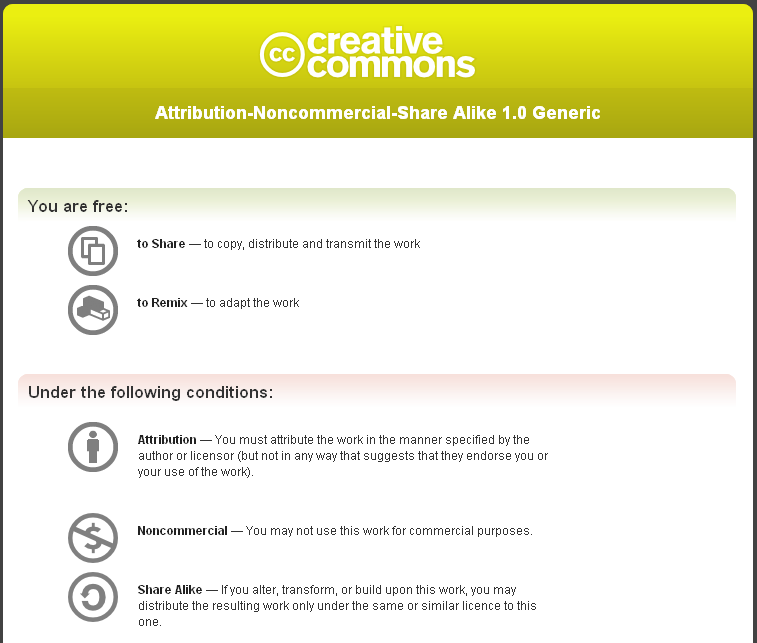
\includegraphics[width=0.6\textwidth]{assets/pics/creative_commons.png}
\begin{tikzpicture}
    \tikzset{node distance = 2.5cm}
    \tikzstyle{every node}=[thick, draw, ellipse, minimum width=100pt,inner sep=10pt,align=center]
    % Nodes
    \node[text width=3.5cm] (node1) {Data Collection};
    \node[text width=3cm] (node2) [right = 2cm of node1] {Data Display};
    \node[text width=2cm, inner sep=5pt,below = 0.3cm and 0.1cm of node1, xshift=3cm] (node3) {Data Reduction};
    \node[rectangle, rounded corners=2mm,text width=6.5cm, below=3.5 cm of node1, xshift=2.4cm] (node4) {Conclusions: drawing/verifying};

    % Arrows
    \draw[-{Latex[length=2mm]}] (node1) -- (node2);
    \draw[-{Latex[length=2mm]}] (node1) -- (node3);
    \draw[{Latex[length=2mm]}-] (node1) -- (node4);
    \draw[{Latex[length=2mm]}-{Latex[length=2mm]}] (node2) -- (node4);
    \draw[{Latex[length=2mm]}-{Latex[length=2mm]}] (node2) -- (node3);
    \draw[{Latex[length=2mm]}-{Latex[length=2mm]}] (node3) -- (node4);

\end{tikzpicture}
{\footnotesize Sumber: \textcite{Sugiyono2008}\par}
\end{figure}

%\clearchapter
%-----------------------------------------------------------------------------%
\chapter{\babEmpat}
%-----------------------------------------------------------------------------%
Apa itu Bab 4?


%-----------------------------------------------------------------------------%
\section{Contoh}
%-----------------------------------------------------------------------------%
\begin{enumerate}
	\item Tahap 1. \\ %\lstinputlisting[language=Python, caption=Contoh kode, label=code:sample2]{assets/4-sample.py}
	Jelaskan %\lst~\ref{code:sample2} di sini.

	\item Tahap 2.
\end{enumerate}

Tulis kesimpulan di sini.

%\clearchapter
%-----------------------------------------------------------------------------%
\chapter{\babLima}
%-----------------------------------------------------------------------------%
Apa itu Bab 5?


%-----------------------------------------------------------------------------%
\section{Contoh}
%-----------------------------------------------------------------------------%
\begin{enumerate}
	\item Nomor 1.
	\item Nomor 2.
\end{enumerate}

\begin{table}
    \onehalfspacing
    \caption{Data informan pada \lokus}
	\begin{center}
	\begin{tabularx}{\textwidth}{|c|X|X|}
    \hline
    \bo{No.} & \bo{Nama} & \bo{Peran} \\ [0.5ex]
    \hline
    1 & \narsumSatu & Pimpinan \lokus~ \\
    \hline
    2 & \narsumDua & Anggota pada \lokus~dan anggota masyarakat \\
    \hline
    3 & \narsumTiga & Pengawas \lokus~ \\ [1ex]
    \hline
    \multicolumn{3}{l}{\footnotesize\textit{Sumber: Catatan penulis}} \\
    \end{tabularx}
    \end{center}
	\label{table:sample}
\end{table}

Tulis penjelasan terkait \tab~\ref{table:sample} di sini.
 % bisa berisi pembahasan bab 4
%\clearchapter
%---------------------------------------------------------------
\chapter{\kesimpulan}
%---------------------------------------------------------------
Pada bab ini, Penulis akan memaparkan kesimpulan penelitian dan saran untuk penelitian berikutnya.


%---------------------------------------------------------------
\section{Kesimpulan}
%---------------------------------------------------------------
Berikut ini adalah kesimpulan terkait pekerjaan yang dilakukan dalam penelitian ini:
\begin{enumerate}
	\item \bo{Poin pertama} \\
	Penjelasan poin pertama.
	\item \bo{Poin kedua} \\
	Penjelasan poin kedua.
\end{enumerate}

Tulis kalimat penutup di sini.


%---------------------------------------------------------------
\section{Saran}
%---------------------------------------------------------------
Berdasarkan hasil penelitian ini, berikut ini adalah saran untuk pengembangan penelitian berikutnya:
\begin{enumerate}
	\item Saran 1.
	\item Saran 2.
\end{enumerate}

%\clearchapter

%
% Daftar Pustaka
% \addChapter{DAFTAR PUSTAKA}
%
% Daftar Pustaka
%

%
% Tambahkan pustaka yang digunakan setelah perintah berikut.
%
\phantomsection %hack to add clickable section for pustaka
\bibliographystyle{ieeetr}
\bibliography{references}

%\clearchapter

% Alternatif manajemen daftar pustaka dengan \bibliography
% \bibliographystyle{apacite}
% \bibliography{src/references}

%
% Lampiran
%
%-----------------------------------------------------------------------------%
\begin{appendix}
% \renewcommand\pagenumbering[1]{} % no numbering
% \renewcommand*{\thepage}{\Roman}
    %
% @author  Andreas Febrian
% @version 1.00
%
% Hanya sebuah pembatas bertuliskan LAMPIRAN ditengah halaman.
%

\begin{titlepage}
	\centering
	\vspace*{6cm}
	\noindent \Huge{LAMPIRAN}
	\addChapter{LAMPIRAN}
\end{titlepage}

%     \clearpage

    \pagestyle{lampiran}
%     \setcounter{page}{2}
%     \chapter{LAMPIRAN}

    \pagenumbering{Roman}
%     \pretocmd{\chapter}{%
%       \clearpage
%       \pagenumbering{Roman}%
%       \renewcommand*{\thepage}{\thechapter\arabic{page}}%
%     }{}{}

  \setlength{\leftskip}{0cm}
%----------------------------------------------------------------------------%

    \newlampiran{Surat Pengantar Penelitian}
%     \centerline{
%         \fbox{ %
%         \parbox{1.05\linewidth}{%
%           \includegraphics[width=\linewidth,trim={2cm 10.5cm 1.5cm 0.5cm},clip]{submission/lampiran_pengantar_penelitian.pdf}
%         %masukkan surat pengantar hasil scan dalam pdf
%           }
%         }
%         }
    \newpage

    % izin penelitian
    \phantomsection
    \newlampiran{Surat Izin Penelitian}
%     \centerline{
%         \frame{\includegraphics[width=1.05\linewidth]{submission/lampiran_surat_izin_penelitian.pdf}}
%         %masukkan surat izin penelitian dari lokasi
%         }
    \newpage


    % pedoman wawancara
    \phantomsection
    \newlampiran{Pedoman Wawancara}
    %
% Lampiran interview Guide
%
% @author  Slamet B. Aryo
% @version 1.10
%

% \newpage
% \pagenumbering{gobble} % enable only for proposal

% \noindent \bo{Lampiran Interview Guide}
\vspace{.5cm}

Berikut adalah pertanyaan wawancara terkait \judul.

\textbf{Kepada Pimpinan}

\begin{enumerate}
    \item Bagaimanakah sejarah berdirinya \lokus?
    \item Apa visi dan misi didirikannya \lokus?
\end{enumerate}

    \newpage

    % traskrip wawancara
    \newlampiran{Transkrip Wawancara}
    %
% Lampiran transkrip interview
%
% @author  Slamet B. Aryo
% @version 1.01
%
\begin{spacing}{1.125}
\noindent \underline{Bapak \narsumSatu~(Kepala \lokus)}

\vspace{1cm}

\begin{enumerate}
\setlength{\itemsep}{12pt}%
\item Bagaimana sejarah berdirinya \lokus?\\
\textit{Jawab:} \lipsum[41-49]

\end{enumerate}
\end{spacing}

    \newpage

    % dokumentasi
    \newlampiran{Dokumentasi}
    %\begin{center}
     \begin{figure}[H]
      \centering
        
\includegraphics[width=0.8\textwidth]{assets/pics/makara.png}
        \caption*{Wawancara dengan \narsumSatu}
     \end{figure}

     \begin{figure}[H]
      \centering
        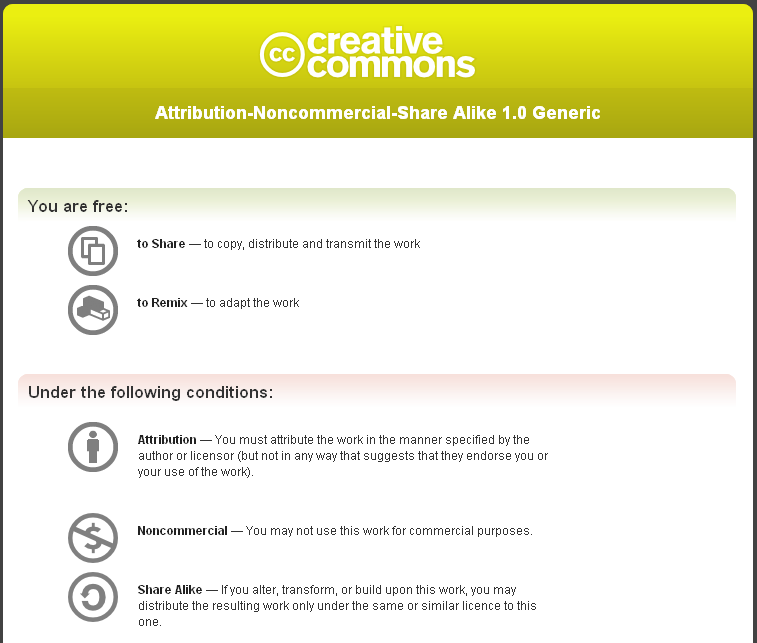
\includegraphics[width=0.8\textwidth]{assets/pics/creative_commons.png}
        \caption*{Wawancara dengan \narsumDua}
     \end{figure}
    %\end{center}
    \newpage


    % riwayat hidup
    \newlampiran{Daftar Riwayat Hidup}
     

    \clearpage
\end{appendix}



\end{document}
